\documentclass{beamer}

\usepackage{beamerthemesplit}
\usetheme{Singapore} %Copenhagen}
%\usecolortheme{whale}

%\usepackage[T2A]{fontenc}
%\usepackage[utf8]{inputenc}
%\usepackage[russian]{babel}

\usepackage[main=russian,english]{babel}   %% загружает пакет многоязыковой вёрстки
\usepackage{fontspec}      %% подготавливает загрузку шрифтов Open Type, True Type и др.
\defaultfontfeatures{Ligatures={TeX},Renderer=Basic}  %% свойства шрифтов по умолчанию
\setmainfont{Times New Roman} %% задаёт основной шрифт документа
%\usefonttheme{professionalfonts}% SOLUTION
\usefonttheme{serif}

\usepackage{hyperref}
\usepackage{textcomp}
\usepackage{amssymb,amsmath}
%\usepackage{animate}
%\usepackage{longtable}
\usepackage{xcolor}

%\usepackage{pgffor}
\usepackage{enumitem}


\newcounter{N}

%% Форматирование окружения itemize
%\usepackage{ragged2e}
%\let\olditem\item
%\renewcommand\item{\olditem\justifying}

\usepackage{ mathrsfs }
\newcommand{\Rho}{\mathscr{P}}

\newcommand{\argxi}{(\xi^1,\xi^2,\xi^3)}
\newcommand{\argx}{(x^1,x^2,x^3)}

\newcommand{\argxiv}{(\vec{\xi})}
\newcommand{\argxv}{(\vec{x})}


\newcommand{\argxbarn}{(\bar{x}^1,\bar{x}^2,\ldots, \bar{x}^n)}
\newcommand{\argxn}{(x^1, x^2,\ldots, x^n)}

\newcommand{\argtxi}{(t, \xi^1,\xi^2,\xi^3)}
\newcommand{\argtoxi}{(t_0, \xi^1,\xi^2,\xi^3)}

\newcommand{\argtxiv}{(t, \vec{\xi})}
\newcommand{\argtoxiv}{(t_0, \vec{\xi})}


\newcommand{\argtx}{(t, x^1,x^2,x^3)}
\newcommand{\argtox}{(t_0, x^1,x^2,x^3)}

\newcommand{\argtxv}{(t, \vec{x})}
\newcommand{\argtoxv}{(t_0, \vec{x})}


\newcommand{\pd}[2]{\frac{\partial #1}{\partial #2}}
\newcommand{\pdk}[2]{\frac{\partial^2 #1}{\partial #2^2}}

\newcommand{\grad}{\operatorname{grad}}
\newcommand{\rot}{\operatorname{rot}}
\newcommand{\divo}{\operatorname{div}}

\title[]{Вихревые течения идеальной жидкости}

\author[]{ {\em Верещагин Антон Сергеевич}
\\
канд. физ.-мат. наук, старший преподаватель\\
\bigskip
Кафедра аэрофизики и газовой динамики ФФ НГУ}

\usebackgroundtemplate{\includegraphics[width=\paperwidth]{../img/background.png}}

\begin{document}
	
\frame{\titlepage}


\frame{
	\frametitle{Аннотация}
	\parbox{\textwidth}{
	
	}
}


\frame{
	\frametitle{ Потенциальные и вихревые течения идеальной жидкости}
	
	\begin{exampleblock}{Определение}
		\parbox{\textwidth}{
			
			Течение идеальной жидкости называется \alert{вихревым}, если вектор $\vec{\Omega} = \rot \vec{v}$ в некоторых точках исследуемой области отличен от нулевого.
					
			\pause	
			Выражение для компонент вектора вихря
			\[
			\Omega_x = \pd{v_z}{y}-\pd{v_y}{z},\quad
			\Omega_y = \pd{v_x}{z}-\pd{v_z}{x},\quad
			\Omega_z = \pd{v_y}{x} -\pd{v_x}{y}.
			\]		
			
			\pause	
			Если же в исследуемой области везде $\vec{\Omega}=0$, тогда течение в этой области называется потенциальным, и существует потенциал $\varphi$ такой, что
			\[
			\vec{v} = \nabla\varphi.
			\]
			Справедливо и обратное утверждение.
			

			
		}
	\end{exampleblock}
	
}

\frame{
	\frametitle{ Пример вихревого течения }
	
	
	\begin{columns}
		\begin{column}{0.5\textwidth}
			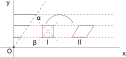
\includegraphics[width=\textwidth]{../img/rot_example.pdf}	
		\end{column}
		\begin{column}{0.5\textwidth}
		Движение жидкости слоями
		\[
		v_x = ay,\quad
		v_y=0,\quad
		v_z=0.
		\]	
		Вихрь скорости 
		\[
			\Omega_x = 0,\quad
			\Omega_y = 0,\quad
			\Omega_z = -a.
		\]
		\end{column}
	\end{columns}

	\begin{exampleblock}{Описание}
		\parbox{\textwidth}{
			По теореме Кельвина-Гельмгольца о скорости деформируемой частицы квадрат $I$  переходит в параллелограмм $II$ посредством сдвига вдоль оси $x$, поворота как твердого тела по указанной стрелке и чистой деформации в виде сжатия вдоль линии $\alpha$ и растяжения вдоль линии $\beta$.
			
		}
	\end{exampleblock}

}

\frame{
	\frametitle{Вихревые линии и вихревые трубки}
	
	\begin{exampleblock}{Определение}
		\parbox{\textwidth}{
			\alert{Вихревой линиией} называется такая линия, во всякой точке которой вихрь скорости $\vec{\Omega}$ направлен по касательной к этой линии. 			
		}
	\end{exampleblock}

	\begin{exampleblock}{Уравнения вихревой линии}
		\parbox{\textwidth}{
			\[
			\frac{dx}{\Omega_x}=\frac{dy}{\Omega_y} = \frac{dz}{\Omega_z}.
			\]
		}
	\end{exampleblock}


}

\frame{
	\frametitle{ Вихревая трубка }
	
	\begin{exampleblock}{Определение}
		\parbox{\textwidth}{
			\alert{Вихревой трубкой} называется совокупность точек пространства, ограниченных вихревыми линиями, проведёнными через заданный замкнуты контур.
		}
	\end{exampleblock}
	
	\bigskip
	\centering
	\includegraphics[width=0.7\textwidth]{../img/rot_tube.pdf}
	

}

\frame{
	\frametitle{ Циркуляция скорости и теорема Стокса}
	
	\begin{exampleblock}{Определение}
		\parbox{\textwidth}{
			\alert{Циркуляцией скорости} $\Gamma$ по замкнутому контуру называется линейный интеграл
			\[
			\Gamma = \oint\limits_C \vec{v}\cdot d\vec{l} = \oint\limits_C v_x dx + v_y dy + v_z dz.
			\]
		}
	\end{exampleblock}
	\begin{exampleblock}{Теорема Стокса}
		\parbox{\textwidth}{
			Циркуляция вектора по замкнутому контуру равна потоку ротора этого вектора через площадку, ограниченную этим контуром:
			\[
			\oint\limits_C \vec{v}\cdot d\vec{l} = 
			\int\limits_S (\vec{n} \cdot \rot \vec{v}) dS,
			\]
			где вектор $\vec{n}$ -- вектор единичной нормали к $S$, направленный по правилу буравчика. 
			
		}
	\end{exampleblock}
}

\frame{
	\frametitle{ Интенсивность вихревой трубки }
	
	\begin{exampleblock}{Определение}
		\parbox{\textwidth}{
			Интенсивностью вихревой трубки называется поток вектора вихря $\Omega$ через сечение вихревой трубки 
			\[
			I=\int\limits_S \vec{\Omega} \cdot \vec{n} dS.
			\]
			
		}
	\end{exampleblock}


}

\frame{
	\frametitle{ Теорема о постоянстве циркуляции для вихревой трубки}
	
	\begin{exampleblock}{Теорема}
		\parbox{\textwidth}{
			Циркуляция скорости по любому замкнутому контуру, охватывающему данную вихревую трубку постоянна.
		}
	
	\bigskip\pause
	\end{exampleblock}
		\begin{columns}
		\begin{column}{0.5\textwidth}
			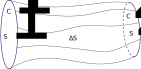
\includegraphics[width=\textwidth]{../img/circul_tube.pdf}
		\end{column}
		\begin{column}{0.5\textwidth}
		\parbox{\textwidth}{
		Рассмотрим вихревую трубку $V$,	ограниченную с торцов сечениями $S_1$, $S_2$ и боковой поверхностью $\Delta S$. Сечения $S_1$, $S_2$ пересекаются с $\Delta S$ по контурам $C_1$ и $C_2$.
		}
		
		\end{column}
	\end{columns}

	\pause
	\bigskip
	\[
	0 = \int\limits_V \divo \rot \vec{v} \, dV= 
	\int\limits_V \divo \vec{\Omega} dV=
	\int\limits_S \vec{\Omega}\cdot \vec{n} dS
	\]
}

\frame{
	\frametitle{ Теорема о постоянстве циркуляции для вихревой трубки: доказательство }
	\centering		
	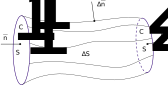
\includegraphics[width=0.5\textwidth]{../img/circul_tube_normals.pdf}
	
	\bigskip
	\parbox{\textwidth}{
	\[
	\int\limits_S \vec{\Omega}\cdot \vec{n} dS = 
	\int\limits_{S_1} \vec{\Omega}\cdot \vec{n}_1 dS+
	\int\limits_{S_2} \vec{\Omega}\cdot \vec{n}_2 dS+
	\int\limits_{\Delta S} \vec{\Omega}\cdot \Delta\vec{n} dS.
	\]	
	Т.к. на боковой поверхности вихревой трубки $\Delta S$ вектора $\vec{\Omega}$ и $\Delta\vec{n}$ ортогональны, то последний интеграл равен 0.
	}
	
	
}


\frame{
	\frametitle{ Теорема о постоянстве циркуляции для вихревой трубки: доказательство }
	\centering		
	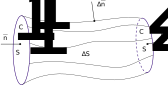
\includegraphics[width=0.5\textwidth]{../img/circul_tube_normals.pdf}
	
	\bigskip
	\parbox{\textwidth}{
		Таким образом, используя теорему Стокса, имеем
		\[
		0 = 
		\int\limits_{S_1} \vec{\Omega}\cdot \vec{n}_1 dS+
		\int\limits_{S_2} \vec{\Omega}\cdot \vec{n}_2 dS=
		\oint\limits_{C_1} \vec{\Omega} \cdot d\vec{l} -
		\oint\limits_{C_2} \vec{\Omega} \cdot d\vec{l}. 	
		\]
		В последнем равенстве появился знак минус, потому что нормали $\vec{n}_1$ и $\vec{n}_2$ направлены в разные стороны. Так как контуры $C_1$ и $C_2$ выбраны произвольно, то справедливо утверждение теоремы. 
	}
	
	
}



\frame{
	\frametitle{ Теорема о постоянстве циркуляции для вихревой трубки: доказательство }
	\centering		
	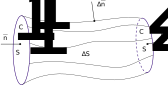
\includegraphics[width=0.5\textwidth]{../img/circul_tube_normals.pdf}
	
	\bigskip
	\parbox{\textwidth}{
		Таким образом, используя теорему Стокса, имеем
		\[
		0 = 
		\int\limits_{S_1} \vec{\Omega}\cdot \vec{n}_1 dS+
		\int\limits_{S_2} \vec{\Omega}\cdot \vec{n}_2 dS=
		\oint\limits_{C_1} \vec{\Omega} \cdot d\vec{l} -
		\oint\limits_{C_2} \vec{\Omega} \cdot d\vec{l}. 	
		\]
		
		Дополнительно показано, что интенсивность вихревой трубки одна и та же в любом сечении. 
	}
	
	
}
\frame{
	\frametitle{ Литература }
	\begin{itemize}[partopsep=1pt,label=\textbullet]
		\item
%		\item {\em Кочин~Н.~Е., Кибель~И.~А., Розе~Н.~В.} Теоретическая гидромеханика. М.:Гос. издат. физ.-мат. лит., 1963.
%		
%		\item {\em Лойцянский~Л.~Г.} Механика жидкости и газ: Учеб. для вузов. -- 7-е изд., испр. М.:Дрофа, 2003.	
		
	\end{itemize}
}
\end{document}
